%% uncomment to list all files in log
%\listfiles

\documentclass[12pt]{report}


\usepackage{fontspec}

%\setmainfont[Scale=MatchLowercase]{Lucida Bright}
%\setmonofont{FreeMono}
%\setmonofont{Source Code Pro}
\setmonofont[Scale=MatchLowercase]{Ubuntu Mono}

\usepackage[headings]{fullpage}

% national use characters 
%\usepackage{inputenc}

% ams mathematical symbols
\usepackage{amsmath,amssymb}

% added to support pandoc highlighting
\usepackage{microtype}

\usepackage{makeidx}

% add index and bibliographies to table of contents
\usepackage[nottoc]{tocbibind}

% postscript courier and times in place of cm fonts
%\usepackage{courier}
%\usepackage{times}

% extended coloring
\usepackage{color}
\usepackage[table,dvipsnames]{xcolor}
\usepackage{colortbl}

% advanced date formating
\usepackage{datetime}

%support pandoc code highlighting
\usepackage{fancyvrb}
\DefineShortVerb[commandchars=\\\{\}]{\|}
\DefineVerbatimEnvironment{Highlighting}{Verbatim}{commandchars=\\\{\}}
% Add ',fontsize=\small' for more characters per line

%tango style colors
% \usepackage{framed}
% \definecolor{shadecolor}{RGB}{255,255,255}
% \newenvironment{Shaded}{\begin{snugshade}}{\end{snugshade}}
% \newcommand{\KeywordTok}[1]{\textcolor[rgb]{0.13,0.29,0.53}{\textbf{{#1}}}}
% \newcommand{\DataTypeTok}[1]{\textcolor[rgb]{0.13,0.29,0.53}{{#1}}}
% \newcommand{\DecValTok}[1]{\textcolor[rgb]{0.00,0.00,0.81}{{#1}}}
% \newcommand{\BaseNTok}[1]{\textcolor[rgb]{0.00,0.00,0.81}{{#1}}}
% \newcommand{\FloatTok}[1]{\textcolor[rgb]{0.00,0.00,0.81}{{#1}}}
% \newcommand{\CharTok}[1]{\textcolor[rgb]{0.31,0.60,0.02}{{#1}}}
% \newcommand{\StringTok}[1]{\textcolor[rgb]{0.31,0.60,0.02}{{#1}}}
% \newcommand{\CommentTok}[1]{\textcolor[rgb]{0.56,0.35,0.01}{\textit{{#1}}}}
% \newcommand{\OtherTok}[1]{\textcolor[rgb]{0.56,0.35,0.01}{{#1}}}
% \newcommand{\AlertTok}[1]{\textcolor[rgb]{0.94,0.16,0.16}{{#1}}}
% \newcommand{\FunctionTok}[1]{\textcolor[rgb]{0.00,0.00,0.00}{{#1}}}
% \newcommand{\RegionMarkerTok}[1]{{#1}}
% \newcommand{\ErrorTok}[1]{\textbf{{#1}}}
% \newcommand{\NormalTok}[1]{{#1}}

%espresso style colors
% \usepackage{framed}
% \definecolor{shadecolor}{RGB}{42,33,28}
% \newenvironment{Shaded}{\begin{snugshade}}{\end{snugshade}}
% \newcommand{\KeywordTok}[1]{\textcolor[rgb]{0.26,0.66,0.93}{\textbf{{#1}}}}
% \newcommand{\DataTypeTok}[1]{\textcolor[rgb]{0.74,0.68,0.62}{\underline{{#1}}}}
% \newcommand{\DecValTok}[1]{\textcolor[rgb]{0.27,0.67,0.26}{{#1}}}
% \newcommand{\BaseNTok}[1]{\textcolor[rgb]{0.27,0.67,0.26}{{#1}}}
% \newcommand{\FloatTok}[1]{\textcolor[rgb]{0.27,0.67,0.26}{{#1}}}
% \newcommand{\CharTok}[1]{\textcolor[rgb]{0.02,0.61,0.04}{{#1}}}
% \newcommand{\StringTok}[1]{\textcolor[rgb]{0.02,0.61,0.04}{{#1}}}
% \newcommand{\CommentTok}[1]{\textcolor[rgb]{0.00,0.40,1.00}{\textit{{#1}}}}
% \newcommand{\OtherTok}[1]{\textcolor[rgb]{0.74,0.68,0.62}{{#1}}}
% \newcommand{\AlertTok}[1]{\textcolor[rgb]{1.00,1.00,0.00}{{#1}}}
% \newcommand{\FunctionTok}[1]{\textcolor[rgb]{1.00,0.58,0.35}{\textbf{{#1}}}}
% \newcommand{\RegionMarkerTok}[1]{\textcolor[rgb]{0.74,0.68,0.62}{{#1}}}
% \newcommand{\ErrorTok}[1]{\textcolor[rgb]{0.74,0.68,0.62}{\textbf{{#1}}}}
% \newcommand{\NormalTok}[1]{\textcolor[rgb]{0.74,0.68,0.62}{{#1}}}

%kete style colors
% \newenvironment{Shaded}{}{}
% \newcommand{\KeywordTok}[1]{\textbf{{#1}}}
% \newcommand{\DataTypeTok}[1]{\textcolor[rgb]{0.50,0.00,0.00}{{#1}}}
% \newcommand{\DecValTok}[1]{\textcolor[rgb]{0.00,0.00,1.00}{{#1}}}
% \newcommand{\BaseNTok}[1]{\textcolor[rgb]{0.00,0.00,1.00}{{#1}}}
% \newcommand{\FloatTok}[1]{\textcolor[rgb]{0.50,0.00,0.50}{{#1}}}
% \newcommand{\CharTok}[1]{\textcolor[rgb]{1.00,0.00,1.00}{{#1}}}
% \newcommand{\StringTok}[1]{\textcolor[rgb]{0.87,0.00,0.00}{{#1}}}
% \newcommand{\CommentTok}[1]{\textcolor[rgb]{0.50,0.50,0.50}{\textit{{#1}}}}
% \newcommand{\OtherTok}[1]{{#1}}
% \newcommand{\AlertTok}[1]{\textcolor[rgb]{0.00,1.00,0.00}{\textbf{{#1}}}}
% \newcommand{\FunctionTok}[1]{\textcolor[rgb]{0.00,0.00,0.50}{{#1}}}
% \newcommand{\RegionMarkerTok}[1]{{#1}}
% \newcommand{\ErrorTok}[1]{\textcolor[rgb]{1.00,0.00,0.00}{\textbf{{#1}}}}
% \newcommand{\NormalTok}[1]{{#1}}
%end pandoc code hacks

% jodliterate colors
\usepackage{color}
\definecolor{shadecolor}{RGB}{248,248,248}
% j control structures 
\definecolor{keywcolor}{rgb}{0.13,0.29,0.53}
% j explicit arguments x y m n u v
\definecolor{datacolor}{rgb}{0.13,0.29,0.53}
% j numbers - all types see j.xml
\definecolor{decvcolor}{rgb}{0.00,0.00,0.81}
\definecolor{basencolor}{rgb}{0.00,0.00,0.81}
\definecolor{floatcolor}{rgb}{0.00,0.00,0.81}
% j local assignments
\definecolor{charcolor}{rgb}{0.31,0.60,0.02}
\definecolor{stringcolor}{rgb}{0.31,0.60,0.02}
\definecolor{commentcolor}{rgb}{0.56,0.35,0.01}
% primitive adverbs and conjunctions
%\definecolor{othercolor}{rgb}{0.56,0.35,0.01}   
\definecolor{othercolor}{RGB}{0,0,255}
% global assignments
\definecolor{alertcolor}{rgb}{0.94,0.16,0.16}
% primitive J verbs and noun names
\definecolor{funccolor}{rgb}{0.00,0.00,0.00}    

\usepackage{framed}
\newenvironment{Shaded}{}{}
\newcommand{\KeywordTok}[1]{\textcolor{keywcolor}{\textbf{{#1}}}}
\newcommand{\DataTypeTok}[1]{\textcolor{datacolor}{{#1}}}
%\newcommand{\DecValTok}[1]{\textcolor{decvcolor}{{#1}}}
\newcommand{\DecValTok}[1]{{#1}} 
\newcommand{\BaseNTok}[1]{\textcolor{basencolor}{{#1}}}
\newcommand{\FloatTok}[1]{\textcolor{floatcolor}{{#1}}}
\newcommand{\CharTok}[1]{\textcolor{charcolor}{\textbf{{#1}}}}
\newcommand{\StringTok}[1]{\textcolor{stringcolor}{{#1}}}
\newcommand{\CommentTok}[1]{\textcolor{commentcolor}{\textit{{#1}}}}
\newcommand{\OtherTok}[1]{\textcolor{othercolor}{{#1}}} 
\newcommand{\AlertTok}[1]{\textcolor{alertcolor}{\textbf{{#1}}}}
%\newcommand{\FunctionTok}[1]{\textcolor{funccolor}{{#1}}}
\newcommand{\FunctionTok}[1]{{#1}}
\newcommand{\RegionMarkerTok}[1]{{#1}}
\newcommand{\ErrorTok}[1]{\textbf{{#1}}}
\newcommand{\NormalTok}[1]{{#1}}

% headers and footers
\usepackage{fancyhdr}
\pagestyle{fancy}

\fancyhead{}
\fancyfoot{}

%\fancyhead[LE,RO]{\slshape \rightmark}
%\fancyhead[LO,RE]{\slshape \leftmark}
\fancyfoot[C]{\thepage}
%\headrulewidth 0.4pt
%\footrulewidth 0 pt

%\addtolength{\headheight}{\baselineskip}

%\lfoot{\emph{Analyze the Data not the Drivel}}
%\rfoot{\emph{\today}}

% subfigure handles figures that contain subfigures
%\usepackage{color,graphicx,subfigure,sidecap}
\usepackage{graphicx,sidecap}
\usepackage{subfigure}
\graphicspath{{./inclusions/}}

% floatflt provides for text wrapping around small figures and tables
\usepackage{floatflt}

% tweak caption formats 
\usepackage{caption} 
\usepackage{sidecap}
%\usepackage{subcaption} % not compatible with subfigure

\usepackage{rotating} % flip tables sideways

% complex footnotes
%\usepackage{bigfoot}

% weird logos \XeLaTeX
\usepackage{metalogo}

% source code listings
\usepackage{listings}

% long tables
% \usepackage{longtable}

\newcommand{\HRule}{\rule{\linewidth}{0.5mm}}

% map LaTeX cross references into PDF cross references
\usepackage[
            %dvips,
            colorlinks,
            linkcolor=blue,
            citecolor=blue,
            urlcolor=blue,   % magenta, cyan default        
            pdfauthor={John D. Baker},
            pdftitle={Analyze the Data not the Drivel},
            pdfsubject={Blog},
            pdfcreator={MikTeX+LaTeXe with hyperref package},
            pdfkeywords={blog,wordpress},
            ]{hyperref}
           
% custom colors
\definecolor{CodeBackGround}{cmyk}{0.0,0.0,0,0.05}    % light gray
\definecolor{CodeComment}{rgb}{0,0.50,0.00}           % dark green {0,0.45,0.08}
\definecolor{TableStripes}{gray}{0.9}                 % odd/even background in tables

\lstdefinelanguage{bat}
{morekeywords={echo,title,pushd,popd,setlocal,endlocal,off,if,not,exist,set,goto,pause},
sensitive=True,
morecomment=[l]{rem}
}

\lstdefinelanguage{jdoc}
{
morekeywords={},
otherkeywords={assert.,break.,continue.,for.,do.,if.,else.,elseif.,return.,select.,end.
,while.,whilst.,throw.,catch.,catchd.,catcht.,try.,case.,fcase.},
sensitive=True,
morecomment=[l]{NB.},
morestring=[b]',
morestring=[d]',
}

% latex size ordering - can never remember it
% \tiny
% \scriptsize
% \footnotesize
% \small
% \normalsize
% \large
% \Large
% \LARGE
% \huge
% \Huge
 
% listings package settings  
\lstset{%
  language=jdoc,                                % j document settings
  basicstyle=\ttfamily\footnotesize,            
  keywordstyle=\bfseries\color{keywcolor}\footnotesize,
  identifierstyle=\color{black},
  commentstyle=\slshape\color{CodeComment},     % colored slanted comments
  stringstyle=\color{red}\ttfamily,
  showstringspaces=false,                       
  %backgroundcolor=\color{CodeBackGround},       
  frame=single,                                
  framesep=1pt,                                 
  framerule=0.8pt,                             
  rulecolor=\color{CodeBackGround},   
  showspaces=false,
  %columns=fullflexible,
  %numbers=left,
  %numberstyle=\footnotesize,
  %numbersep=9pt,
  tabsize=2,
  showtabs=false,
  captionpos=b
  breaklines=true,                              
  breakindent=5pt                              
}

\lstdefinelanguage{JavaScript}{
  keywords={typeof, new, true, false, catch, function, return, null, catch, switch, var, if, in, while, do, else, case, break},
  ndkeywords={class, export, boolean, throw, implements, import, this},
  ndkeywordstyle=\color{darkgray}\bfseries,
  sensitive=false,
  comment=[l]{//},
  morecomment=[s]{/*}{*/},
  morestring=[b]',
  morestring=[b]"
}

% C# settings
\lstdefinestyle{sharpc}{
language=[Sharp]C,
basicstyle=\ttfamily\scriptsize, 
keywordstyle=\bfseries\color{keywcolor}\scriptsize,
framerule=0pt
}

% for source code listing longer than two use smaller font
\lstdefinestyle{smallersource}{
basicstyle=\ttfamily\scriptsize, 
keywordstyle=\bfseries\color{keywcolor}\scriptsize,
framerule=0pt
}

\lstdefinestyle{resetdefaults}{
language=jdoc,
basicstyle=\ttfamily\footnotesize,  
keywordstyle=\bfseries\color{keywcolor}\footnotesize,                                                               
framerule=0.8pt 
}

% APL UTF8 code points listed for lstlisting processing
\makeatletter
\lst@InputCatcodes
\def\lst@DefEC{%
 \lst@CCECUse \lst@ProcessLetter
  ^^80^^81^^82^^83^^84^^85^^86^^87^^88^^89^^8a^^8b^^8c^^8d^^8e^^8f%
  ^^90^^91^^92^^93^^94^^95^^96^^97^^98^^99^^9a^^9b^^9c^^9d^^9e^^9f%
  ^^a0^^a1^^a2^^a3^^a4^^a5^^a6^^a7^^a8^^a9^^aa^^ab^^ac^^ad^^ae^^af%
  ^^b0^^b1^^b2^^b3^^b4^^b5^^b6^^b7^^b8^^b9^^ba^^bb^^bc^^bd^^be^^bf%
  ^^c0^^c1^^c2^^c3^^c4^^c5^^c6^^c7^^c8^^c9^^ca^^cb^^cc^^cd^^ce^^cf%
  ^^d0^^d1^^d2^^d3^^d4^^d5^^d6^^d7^^d8^^d9^^da^^db^^dc^^dd^^de^^df%
  ^^e0^^e1^^e2^^e3^^e4^^e5^^e6^^e7^^e8^^e9^^ea^^eb^^ec^^ed^^ee^^ef%
  ^^f0^^f1^^f2^^f3^^f4^^f5^^f6^^f7^^f8^^f9^^fa^^fb^^fc^^fd^^fe^^ff%
  ^^^^20ac^^^^0153^^^^0152%
  ^^^^20a7^^^^2190^^^^2191^^^^2192^^^^2193^^^^2206^^^^2207^^^^220a%
  ^^^^2218^^^^2228^^^^2229^^^^222a^^^^2235^^^^223c^^^^2260^^^^2261%
  ^^^^2262^^^^2264^^^^2265^^^^2282^^^^2283^^^^2296^^^^22a2^^^^22a3%
  ^^^^22a4^^^^22a5^^^^22c4^^^^2308^^^^230a^^^^2336^^^^2337^^^^2339%
  ^^^^233b^^^^233d^^^^233f^^^^2340^^^^2342^^^^2347^^^^2348^^^^2349%
  ^^^^234b^^^^234e^^^^2350^^^^2352^^^^2355^^^^2357^^^^2359^^^^235d%
  ^^^^235e^^^^235f^^^^2361^^^^2362^^^^2363^^^^2364^^^^2365^^^^2368%
  ^^^^236a^^^^236b^^^^236c^^^^2371^^^^2372^^^^2373^^^^2374^^^^2375%
  ^^^^2377^^^^2378^^^^237a^^^^2395^^^^25af^^^^25ca^^^^25cb%  
  ^^00}
\lst@RestoreCatcodes
\makeatother

% custom lengths used within minipages
\newcommand{\minindent}{17pt}


\makeindex

\begin{document}

\subsection*{\href{https://analyzethedatanotthedrivel.org/2017/04/30/what-is-required-citizen-environment-sampling-drones/}{What is Required: Citizen Environment Sampling Drones}}
\addcontentsline{toc}{subsection}{What is Required: Citizen Environment Sampling Drones}


\noindent\emph{Posted: 01 May 2017 00:34:14}
\vspace{6pt}

We are well into the drone age. Not long ago drones served only
deep-pocketed governments and corporations. This is still the case.
Whenever you hear about drone strikes on wedding parties, oops terrorist
gatherings, the ``responsible'' drone is probably a standard overpriced
multimillion dollar product of the military industrial crony complex.
Why dispatch terrorists with a few bullets when you can spend millions
of newly created and freshly taxed dollars instead? War may be hell but
business is business.

If things had been left to the druthers of the crony crowd the cozy
world of cost-plus drones would have lasted forever but then technology
happened. Remember those annoying toy quadcopters that flew around the
atriums of shopping malls just a few years ago. You probably thought,
``That's a cute toy'' Well those cheap little toys have grown up and are
now
\href{http://www.popularmechanics.com/flight/drones/a25282/flame-throwing-drones/}{cleaning
power lines with flame throwers},
\href{http://dailycaller.com/2016/03/30/narco-drones-the-cartels-newest-tech-savvy-smuggling-sop-spooks-security-experts/}{carrying
drugs across borders},\footnote{The advent of drones highlights the utter stupidity of Trump's border
wall. How high will the wall have to be to stop drones from flying
over it? How many anti-drone-drones will need to be stationed along
the wall to secure the border?} %\protect\hyperlink{fn1}{\textsuperscript{1}}
\href{https://www.washingtonpost.com/local/prisons-try-to-stop-drones-from-delivering-drugs-porn-and-cellphones-to-inmates/2016/10/12/645fb102-800c-11e6-8d0c-fb6c00c90481_story.html}{smuggling
contraband into prisons},
\href{https://www.youtube.com/watch?v=vdgvlHH3JSA}{annoying eagles},
\href{http://nypost.com/2017/03/16/war-against-isis-now-involves-shuttlecock-grenades-dropped-by-drones/}{dropping
grenades on ISIS}, and
\href{https://www.youtube.com/watch?v=FZOgy5V9imI}{taking really great
selfies}.


%{[}caption id=``attachment\_5366'' align=``aligncenter''  width=``300''{]}
%\href{w.popularmechanics.com/flight/drones/a25282/flame-throwing-drones/}{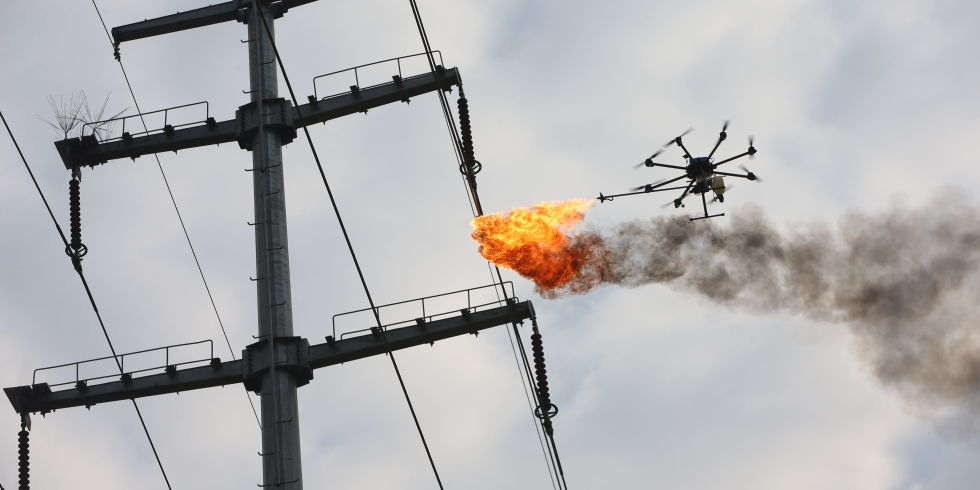
\includegraphics[width=3.12500in,height=1.56250in]{https://bakerjd99.files.wordpress.com/2017/04/flame-drone.jpg?w=300}}
%It's an airborne ``Drone-cue.'' ~The age of the drone is just getting
%started. These gadgets will be put to all sorts of uses. Monitoring the
%environment, with or without the permission of authorities, is an
%excellent use of drones.
%{[}/caption{]}

\captionsetup[figure]{labelformat=empty}
%\begin{figure}[htbp]
\begin{SCfigure}
\centering
\href{www.popularmechanics.com/flight/drones/a25282/flame-throwing-drones/}{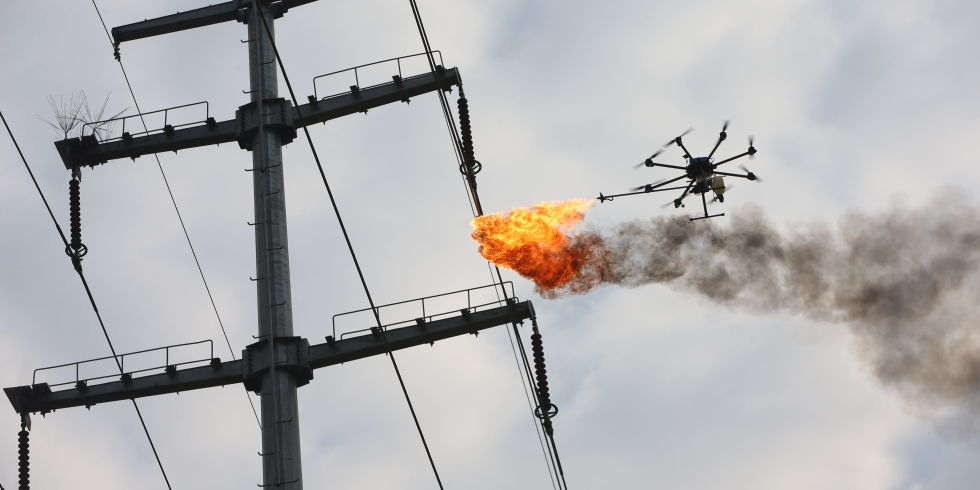
\includegraphics[width=0.40\textwidth]{flame-drone.jpg}}
\caption{It's an airborne ``Drone-cue.'' The age of the drone is just getting
started. These gadgets will be put to all sorts of uses. Monitoring the
environment, with or without the permission of authorities, is an
excellent use of drones.}
\label{fig:5375X0}
\end{SCfigure}
%\end{figure}


Small inexpensive drones are being put to so many creative uses that
it's beginning to worry our self-appointed overlords. You don't need
crony connections and millions of dollars to launch drone attacks. Any
moron with an iPhone and a drone can declare war on the ruling classes.
Not many see it but we're entering a golden age of drone assassins.
Small drones will continue to improve and diversify. They will fly
further, faster and quieter. They will creep, climb, tunnel and bore
through any obstacle. Whatever silly government legislation and
anti-drone measures authorities concoct will be quickly countered and
worked around. The drone genie, like strong encryption before it, is out
of the bottle and it isn't going back in. \emph{Basically, if you're
somebody that needs killing a drone is being assigned your number right
now.}

As much as I enjoy drone enabled asshole termination that's not what I
am requiring today. If you've been paying attention to what's precisely
labeled ``fake news'' you've probably noticed that a strange tweeting
orange ogre has moved into the White House. Yes, it's the end of the
world. One of the ogre's first outrages was to appoint like-minded ogres
to allegedly important government posts. Imagine that!

Of great concern to ``so-called'' environmentalists is the ogre
appointed to behead the \href{https://www.epa.gov/}{EPA}. This cruel EPA
slayer is not drinking the Earth first Kool-Aid and appears determined
to end the cushy pensioned sinecures of all the left-thinking,
environment protecting, comrades. Like I said before, it's the end of
the world. Apparently, after a few, and I mean a very few,
underperforming EPA comrades are purged this critical government agency
will become deaf, dumb and
blind.\footnote{Considering that the EPA is already deaf and dumb how bad can blind be?} %\protect\hyperlink{fn2}{\textsuperscript{2}} 
All that wonderful
EPA air and water quality data will no longer be collected. Only large
infusions of newly created and freshly taxed money can prevent this
apocalypse.

For Christ sakes, cry me an orange river!


%{[}caption id=``attachment\_5367'' align=``aligncenter''  width=``400''{]}
%\href{https://www.wired.com/2015/08/epa-accidentally-turned-river-toxicand-orange/}{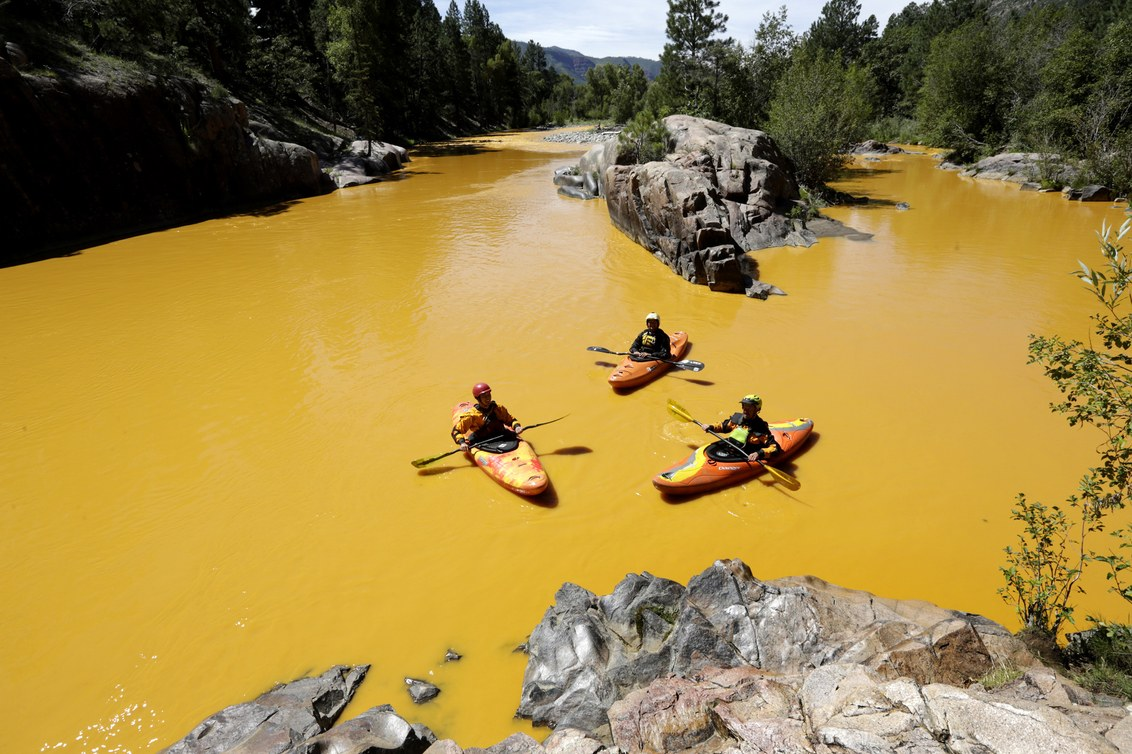
\includegraphics[width=4.16667in,height=2.77083in]{https://bakerjd99.files.wordpress.com/2017/04/orange-river.jpg?w=584}}
%Critics of Trump's appointment of Scott Pruitt to head the EPA should
%keep in mind that the bar for ``wrecking'' the EPA has been set very low
%by the Obama administration. It was the EPA that turned the Animas River
%orange. Yes, it was an unfortunate accident, and sometimes you have to
%destroy the river in order to save it. Two states and the Navajo Nation
%are suing the EPA for gross negligence and incompetence and based on
%images like this I'm guessing they have a case.
%{[}/caption{]}


%\begin{figure}[htbp]
\begin{SCfigure}
\centering
\href{https://www.wired.com/2015/08/epa-accidentally-turned-river-toxicand-orange/}{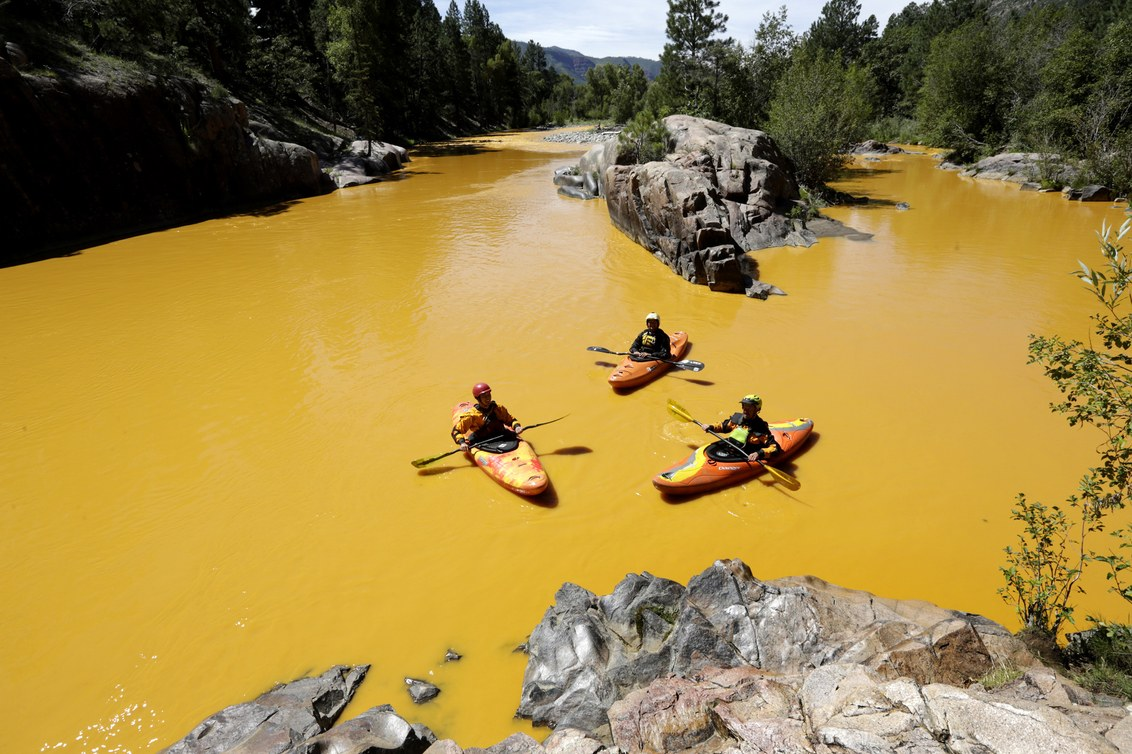
\includegraphics[width=0.50\textwidth]{orange-river.jpg}}
\caption{Critics of Trump's appointment of Scott Pruitt to head the EPA should
keep in mind that the bar for ``wrecking'' the EPA has been set very low
by the Obama administration. It was the EPA that turned the Animas River
orange. Yes, it was an unfortunate accident, and sometimes you have to
destroy the river in order to save it. Two states and the Navajo Nation
are suing the EPA for gross negligence and incompetence and based on
images like this I'm guessing they have a case.}
\label{fig:5375X1}
\end{SCfigure}
%\end{figure}


If you really care about the environment get off your fat corn syrup
enlarged ass and collect your own data with drones. I've listened to
\emph{cis-lefties} insist they are smarter, fitter and better looking
than their evil \emph{cis-righty} counterparts for years. Well, here's
an opportunity to prove it. Instead of marching for science why don't
you modify or build drones that can actually do science.

One of my favorite scenes in the movie
\href{https://en.wikipedia.org/wiki/Erin_Brockovich_(film)}{\emph{Erin
Brockovich}} shows our spunky girl-power heroine played by Julia
Roberts\footnote{I admit it; I've seen too many Julia Roberts movies. Like many mainly
manly men, I have a thing for nice smiles and boobs and no amount of
feminist nagging will change that.} %\protect\hyperlink{fn3}{\textsuperscript{3}} 
sneaking onto~the
grounds of a power plant to clandestinely sample waste water ponds. She
was caught and shooed away but not before she snagged water samples that
contained Hexavalent Chromium: the same, \emph{unnaturally occurring},
compound that also turned up in the drinking water of people living near
the plant. What a coincidence? Erin may have been a spunky go getter but
chemistry was the real hero.

Erin was taking a real risk sneaking onto ``private property.'' In many
parts of the world, she would have been shot and dumped into the
wastewater ponds. How many of us would take such a risk? If only there
was a way to reduce the risks of clandestine sampling. If only there was
a small, hard to detect, quiet, remote-controlled device that could fly
into ``forbidden zones'', sample areas of interest, and then fly out
with physical evidence.

It wouldn't be all that difficult to modify existing drones to do this.
It would make a great science fair project. Think of how much better
things would be if pinheaded SJWs stopped
\href{http://ageofshitlords.com/complete-list-of-all-tumblr-sexualities-so-far}{enumerating
new imaginary genders} and devoted their time and energy to mastering
the technology required to build and operate sampling drones. Instead of
being an embarrassing stain on humanity they might actually do some
good.

Finally, combine clandestine drone sampling with
\href{https://lbry.io/learn}{blockchain based unbannable binary file
distribution} and it's possible to create the type of ``transparency''
political buttheads are always blathering about but never actually
provide.

%\begin{center}\rule{0.5\linewidth}{\linethickness}\end{center}
%
%\begin{enumerate}
%\item
%  \hypertarget{fn1}{}
%
%  The advent of drones highlights the utter stupidity of Trump's border
%  wall. How high will the wall have to be to stop drones from flying
%  over it? How many anti-drone-drones will need to be stationed along
%  the wall to secure the border?\protect\hyperlink{fnref1}{↩}
%\item
%  \hypertarget{fn2}{}
%
%  Considering that the EPA is already deaf and dumb how bad can blind
%  be?\protect\hyperlink{fnref2}{↩}
%\item
%  \hypertarget{fn3}{}
%
%  I admit it; I've seen too many Julia Roberts movies. Like many mainly
%  manly men, I have a thing for nice smiles and boobs and no amount of
%  feminist nagging will change that.\protect\hyperlink{fnref3}{↩}
%\end{enumerate}



%\end{document}